\section{State of The Art}

Example of including a picture
\begin{figure}[htbp]
	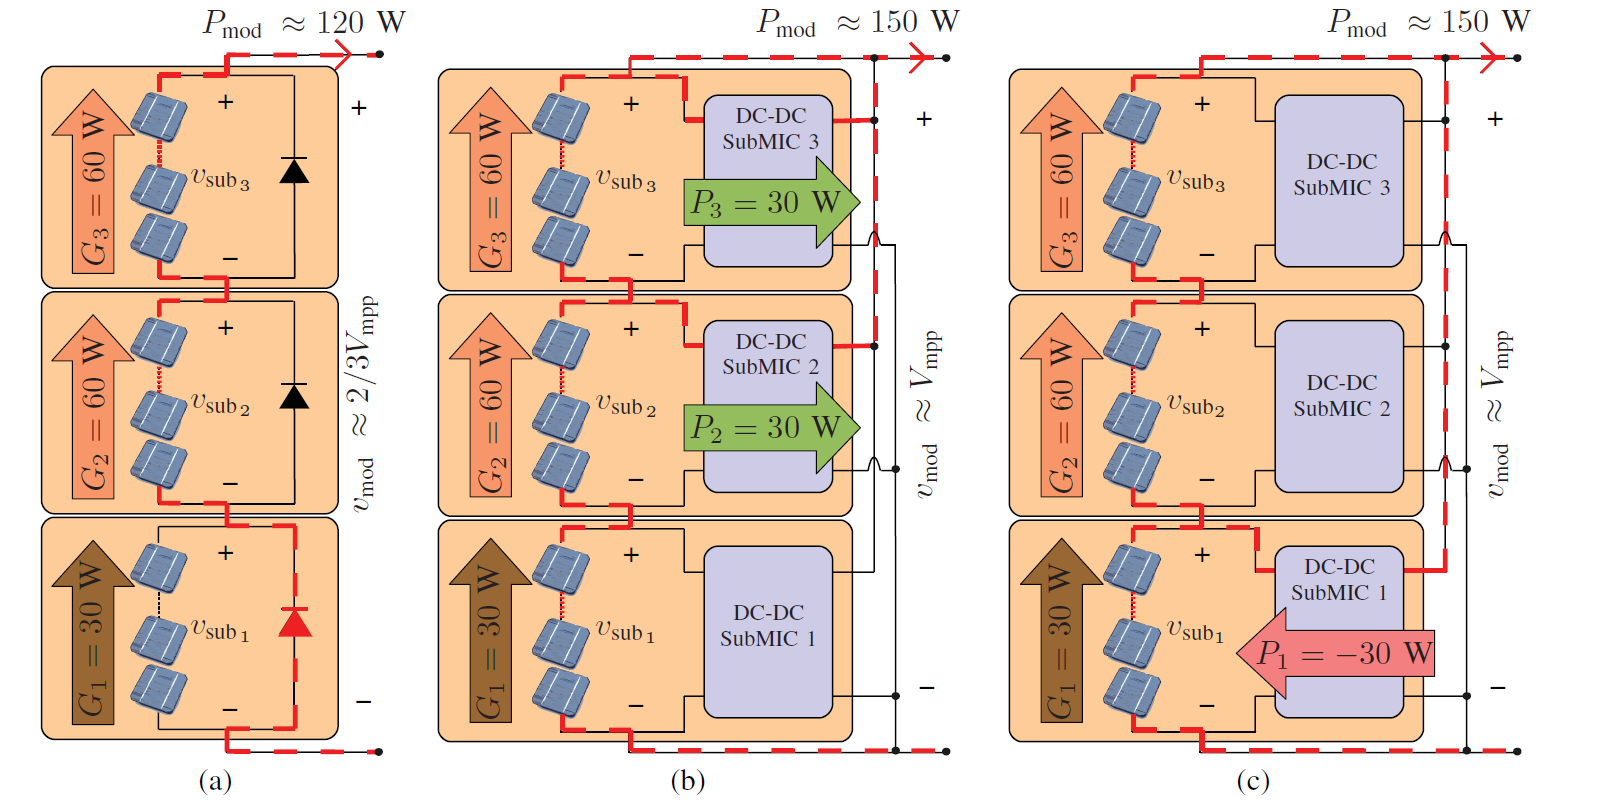
\includegraphics[width=\linewidth]{../Pictures/test.png}
	\caption{Functional flow block diagram}
	\label{fig:TimePlan}
\end{figure}

Example of creating a table \ref{table}.
\begin{table}[htbp]
	\begin{tabular}{|m{1.5cm}|m{8cm}|m{2.5cm}|m{2.5cm}|}
		\hline
		\rowcolor{lightgray} \textbf{ID} & \textbf{Technical Requirements}  & \textbf{Requirement Type}  &  \textbf{Verification Method}    \\ \hline
		AX-1 & The pod shall be center-mountable on the Royal Danish Air Force (RDAF) F-16 AM/BM fighter aircrafts in version M6.5     & M   & A      \\ \hline
		\rowcolor{Seashell2} AX-2 & The pod shall have a mass less than 700 pounds in total & M  & A        \\ \hline
		AX-3 & The pod shall have a geometric cross-section of $0.40m^2$  or less as seen from the front   &  M   & A                \\ \hline
		\rowcolor{Seashell2} AX-4 & The pod should have a geometric cross-section of $0.25m^2$ or less as seen from the front   &  D   &                \\ \hline
	\end{tabular}
	\caption{Flight requirements}
	\label{table}
\end{table}